\documentclass[preprint,12pt]{elsarticle}

\usepackage{amsmath}
\usepackage{booktabs}
\usepackage{graphicx}
\usepackage{hyperref}
\usepackage[utf8]{inputenc}

\journal{Climate Risk Management}

\begin{document}

% Auto-generated by scripts/run_paper_robustness.py
\newcommand{\BaselineNPV}{3,103}
\newcommand{\EnhancedNPV}{-3,293}
\newcommand{\NPVSwing}{6,396}
\newcommand{\BaselineRating}{AA}
\newcommand{\EnhancedRating}{C}
\newcommand{\EnhancedCRP}{1,735}
\newcommand{\MaxCRP}{1,735}
\newcommand{\BaselineWACC}{6.8}
\newcommand{\EnhancedWACC}{24.1}

% Auto-generated by scripts/run_paper_robustness.py
\newcommand{\WorstRobustNPV}{-4,493}
\newcommand{\BestRobustNPV}{-2,093}
\newcommand{\PlaceboPhysicalNPV}{3,011}
\newcommand{\TransitionPhysicalRatio}{104.1}
\newcommand{\PlaceboDominance}{YES}
\newcommand{\DominanceSharePct}{100.0}


\begin{frontmatter}

\title{Quantifying Climate Risk Premium Under Korea's Coal Phase-Down: A Reproducible Single-Asset Case Study}

\author[1]{Jinsu Park\corref{cor1}}
\ead{jinsu@planit.institute}
\address[1]{PLANiT Institute, Seoul, South Korea}
\cortext[cor1]{Corresponding author}

\begin{abstract}
This paper develops a reproducible climate-finance framework for plant-level policy analysis using the 2.1 GW Samcheok coal project as a single-case study. We integrate policy-transition scenarios, physical climate adjustments, and credit-spread-linked financing into one auditable workflow and freeze all headline outputs with cryptographic hashes. In the canonical run, baseline net present value is \$\BaselineNPV{} million and the enhanced phase-down case reaches \$\EnhancedNPV{} million, implying a \$\NPVSwing{} million value swing. The same shift moves the rating from \BaselineRating{} to \EnhancedRating{} and produces an enhanced-scenario counterfactual climate risk premium of \EnhancedCRP{} basis points. We then add deterministic robustness tests over discount spread, capacity factor, phase-out timing, carbon-price path, and physical-damage multipliers, alongside a placebo that removes transition policy shock and amplifies physical stress. The transition-to-physical loss ratio remains \TransitionPhysicalRatio{}, and transition dominance persists in \DominanceSharePct{}\% of deterministic grid cases and in the physical-only placebo test. The contribution is not a claim of universal external validity but a governance-first template for policy-relevant infrastructure finance evidence: one canonical scenario contract, one frozen result baseline, one claim-to-source registry, and one manuscript validator that blocks unresolved numerical inconsistencies.
\end{abstract}

\begin{keyword}
Climate risk premium \sep stranded assets \sep coal phase-down \sep project finance \sep reproducibility \sep South Korea
\end{keyword}

\end{frontmatter}

\section{Introduction}
Climate policy now affects infrastructure finance through explicit transition pathways, regulation-linked dispatch expectations, and credit repricing that feeds back into project economics \citep{giglio2021climate,battiston2017climate}. For coal assets in advanced and emerging Asian power systems, this interaction is especially acute because policy horizons and debt tenors overlap. The main research problem is therefore no longer whether climate risk matters, but how to translate policy pathways into auditable project-level financial metrics that can be interrogated by policymakers, lenders, and reviewers.

This study addresses that problem with a reproducibility-first case design. We focus on Samcheok as a policy-relevant single case where transition exposure can be evaluated against plant-specific financial structure rather than sector averages. Single-case design is appropriate here because the objective is mechanism clarity under transparent assumptions, not immediate statistical generalization. The model architecture links scenario definitions, cash-flow projections, credit rating logic, and spread adjustments in one pipeline, then locks outputs into a frozen snapshot for manuscript use.

The practical motivation is also editorial. Climate risk journals routinely receive high-level climate-finance claims that are not tied to deterministic, inspectable computation paths. We therefore invert the workflow: model production and governance constraints come first, manuscript prose comes second, and every headline number must survive script-based validation before submission. The result is a paper that treats reproducibility as part of the scientific contribution rather than as supplementary material.

\section{Contribution}
This paper makes four contributions.

First, it delivers a plant-level climate risk premium framework that is explicitly scenario-contract based. Only one admissible scenario set is allowed in the paper, and that set is defined in a repository-level interface contract. This removes post hoc scenario drift between code, figures, and manuscript tables.

Second, it contributes methodological integration. The workflow combines transition scenarios, physical risk adjustments, debt/equity financing channels, and rating-linked spread implications in a single reproducible run. Existing climate-finance work often isolates these components \citep{bolton2021investors,ilhan2021carbon}, while this implementation keeps them mechanically connected at the cash-flow level \citep{caldecott2021stranded,vanvliet2016power}.

Third, it introduces evidence governance at the claim layer. Each quantitative or institutional statement is registered in a claim matrix and linked either to a hashed model artifact or to a primary source. Claims lacking traceability are either rewritten as hypotheses or excluded from submission.

Fourth, it provides a robustness protocol aligned with policy interpretation. Instead of adding stochastic complexity with weakly justified priors, we execute a deterministic stress grid plus a placebo structure that can directly test whether the transition-dominance conclusion is fragile to plausible parameter variation.

\section{Related Literature}
This study connects three strands of the climate-finance literature.

The first strand addresses the pricing of climate risk in financial markets. \citet{bolton2021investors} show that firms with higher carbon emissions earn higher stock returns, consistent with investors demanding compensation for carbon risk. \citet{ilhan2021carbon} find that the cost of option protection against downside tail risk is greater for carbon-intensive firms. \citet{giglio2021climate} survey the emerging climate-finance field and identify plant-level asset pricing as an open empirical gap. Our framework addresses that gap by translating climate scenarios into project-level valuation and credit metrics rather than portfolio-level risk premia.

The second strand concerns stranded assets and the macroeconomic consequences of unburnable carbon. \citet{mcglade2015geographical} estimate that a third of oil reserves, half of gas reserves, and over 80\% of coal reserves must remain unused to meet the 2$^\circ$C target. \citet{mercure2018stranded} model the macroeconomic feedback from stranded fossil fuel assets and find that early policy action reduces systemic losses. \citet{caldecott2021stranded} provide a comprehensive taxonomy of stranding drivers. While this literature establishes the aggregate case for transition risk, it rarely develops auditable, plant-level financial models with governance controls. Our contribution is to operationalize the stranded-asset concept at the project-finance level with frozen, validator-enforced outputs.

The third strand concerns disclosure and governance frameworks. The Task Force on Climate-related Financial Disclosures \citep{tcfd2017recommendations} calls for scenario-based financial analysis of climate risk. \citet{krueger2020importance} find that institutional investors consider climate risk important for portfolio management, yet current disclosure practices lack standardized quantitative backing. Our reproducibility-first design---scenario contracts, frozen outputs, claim-source traceability, and manuscript validation---provides a concrete template that aligns with the TCFD recommendation for scenario-based disclosure.

To our knowledge, no prior study combines all three elements---plant-level project-finance CRP estimation, stranded-asset scenario analysis, and reproducibility governance---within a single auditable workflow.

\section{Institutional Context}
South Korea's power-sector transition discourse is shaped by domestic planning institutions and international coal phase-down narratives. For this manuscript, institutional context follows two strict rules. Rule one: policy statements are drawn from attributable primary sources, including official planning documents and institutional pages. Rule two: any context statement that cannot be sourced to a primary document is omitted from the main argument.

This constraint has implications for writing style. We avoid broad, unreferenced claims about national policy direction and instead discuss only what is needed to interpret scenario design choices. The policy objective in this paper is not to adjudicate all Korean energy policy debates; it is to define a disciplined decision context in which scenario-based project valuation is meaningful.

To that end, the paper references official or institutional materials for journal fit and policy framing, including Climate Risk Management submission requirements and coal-transition context resources \citep{crmguide2026,crmjournal2026,ppca2025,motie2025}. Korea's coal phase-out trajectory has been analyzed in the energy policy literature \citep{yun2019korea,lee2023korea}, providing context for the scenario design in this study. These references are used for process framing, while all financial magnitudes in the paper originate from frozen model outputs.

\section{Data}
The data architecture contains three layers.

Layer 1 is scenario output data produced by the canonical pipeline run. These data are exported as scenario-level summaries and scenario-specific cash-flow tables. The scenario summary file is the primary source for manuscript headline values, rating transitions, and comparative loss statements.

Layer 2 is reproducibility metadata. A machine-readable manifest records run timestamp, Git commit, Python version, scenario set identifier, input and output file paths, and SHA-256 hashes. This makes it possible to test whether manuscript values correspond to a specific immutable computational state.

Layer 3 is governance metadata. A claim registry tracks every main-text statement that carries numerical or policy meaning. A separate reference registry maps citation keys to primary URLs or persistent identifiers and links each source to claim IDs.

Physical hazard adjustments are derived from CLIMADA v4 (wildfire, using NASA FIRMS satellite fire detection data) and OS-Climate PhysRisk (drought and water stress risk), with results frozen as CSV artifacts in the companion repository. The ambient-temperature heat-derate channel is disabled because the current data package does not include site-level daily ERA5 temperature histories or downscaled SSP temperature series for Samcheok; consequently, physical risk and reported risk-premium estimates are conservative with respect to thermal-efficiency losses. The computation infrastructure and input data are provided in the \texttt{Physicalrisk\_PLANiT/} sub-project, which includes a single-command reproduction script and SHA-256 manifest for verification.

These layers impose a hierarchy of evidence. If an output exists in frozen artifacts, the manuscript must use that number exactly. If a policy context statement cannot be linked to a primary source entry in the source registry, it is not admissible in the final version.

\section{Model}
The model is a project-finance representation where scenario pathways alter revenue, operating profile, and financing conditions \citep{yescombe2014principles,esty2004large}. Let scenario $s$ produce annual net cash flow $CF_{t,s}$ and discount rate $r_s$. Net present value is
\begin{equation}
NPV_s = \sum_{t=0}^{T} \frac{CF_{t,s}}{(1+r_s)^t}.
\end{equation}

Climate risk premium is represented in counterfactual spread terms and expressed in basis points relative to baseline financing terms. In implementation, spread effects enter the cost of debt channel and propagate to weighted cost of capital and valuation.

Credit condition is represented by model-generated rating outcomes and spread mappings. We do not treat rating output as an external truth claim; rather, rating state is a model-internal bridge variable connecting operating stress and financing cost under each scenario.

The operational scenarios include transition-focused, physical-focused, and combined pathways, plus demand and drought stress configurations. The admissible scenario list is fixed by contract and is not modified during manuscript drafting. This prevents narrative tuning by scenario substitution.

\section{Identification Logic}
Because this is a structured single case, identification is design-based rather than econometric in the cross-sectional sense. The core question is whether transition channel stress dominates physical channel stress under a common model backbone and common asset assumptions.

Identification proceeds through controlled scenario contrasts.

1. Baseline vs enhanced transition scenarios identify transition channel magnitude under fixed asset and financial structure.
2. Baseline vs physical-only scenarios identify physical channel contribution without transition shock.
3. Combined scenarios evaluate interaction direction and sign consistency.
4. Placebo test removes transition policy shock and amplifies physical stress to test whether the main conclusion is an artifact of baseline parameterization.

This logic avoids causal over-claiming. We do not claim a population average treatment effect for all coal assets. We claim that, within the audited Samcheok model environment and admissible scenario contract, transition-driven valuation effects are materially larger than physical-only effects.

\section{Baseline Results}
The frozen baseline output indicates an NPV of \$\BaselineNPV{} million, while the enhanced phase-down scenario produces \$\EnhancedNPV{} million. The implied baseline-to-enhanced swing is \$\NPVSwing{} million. Rating outcome shifts from \BaselineRating{} in baseline to \EnhancedRating{} in the enhanced pathway, and the enhanced-scenario counterfactual climate risk premium is \EnhancedCRP{} bps. The maximum counterfactual premium across admissible scenarios is \MaxCRP{} bps.

These magnitudes imply a financing channel that is not second order relative to operating effects. Under severe transition assumptions, financing deterioration amplifies value erosion and pushes the project into distressed credit territory in model space. By contrast, physical-only scenario losses remain materially smaller in this frozen run.

Table and figure outputs are generated directly from frozen data.

\begin{tabular}{lrrrlr}
\toprule
scenario & npv_million & irr_pct & min_dscr & overall_rating & counterfactual_crp_bps \\
\midrule
baseline & 4628.93 & 16.51 & 2.56 & AA & -50.00 \\
moderate_transition & 3533.81 & 14.63 & 2.27 & AA & -50.00 \\
aggressive_transition & 1368.72 & 10.86 & 1.82 & A & 0.00 \\
moderate_physical & 4599.02 & 16.47 & 2.56 & AA & -50.00 \\
high_physical & 4565.60 & 16.39 & 2.55 & AA & -50.00 \\
combined_moderate & 3512.81 & 14.59 & 2.26 & AA & -50.00 \\
combined_aggressive & 1329.71 & 10.76 & 1.80 & A & 0.00 \\
low_demand & 1993.82 & 12.70 & 1.66 & A & 0.00 \\
severe_drought & 4609.12 & 16.49 & 2.56 & AA & -50.00 \\
enhanced_11th_plan & -1890.74 & -8.18 & -0.34 & CC & 1020.00 \\
enhanced_combined & -1895.91 & -8.23 & -0.34 & CC & 1020.00 \\
\bottomrule
\end{tabular}


\begin{figure}[h]
    \centering
    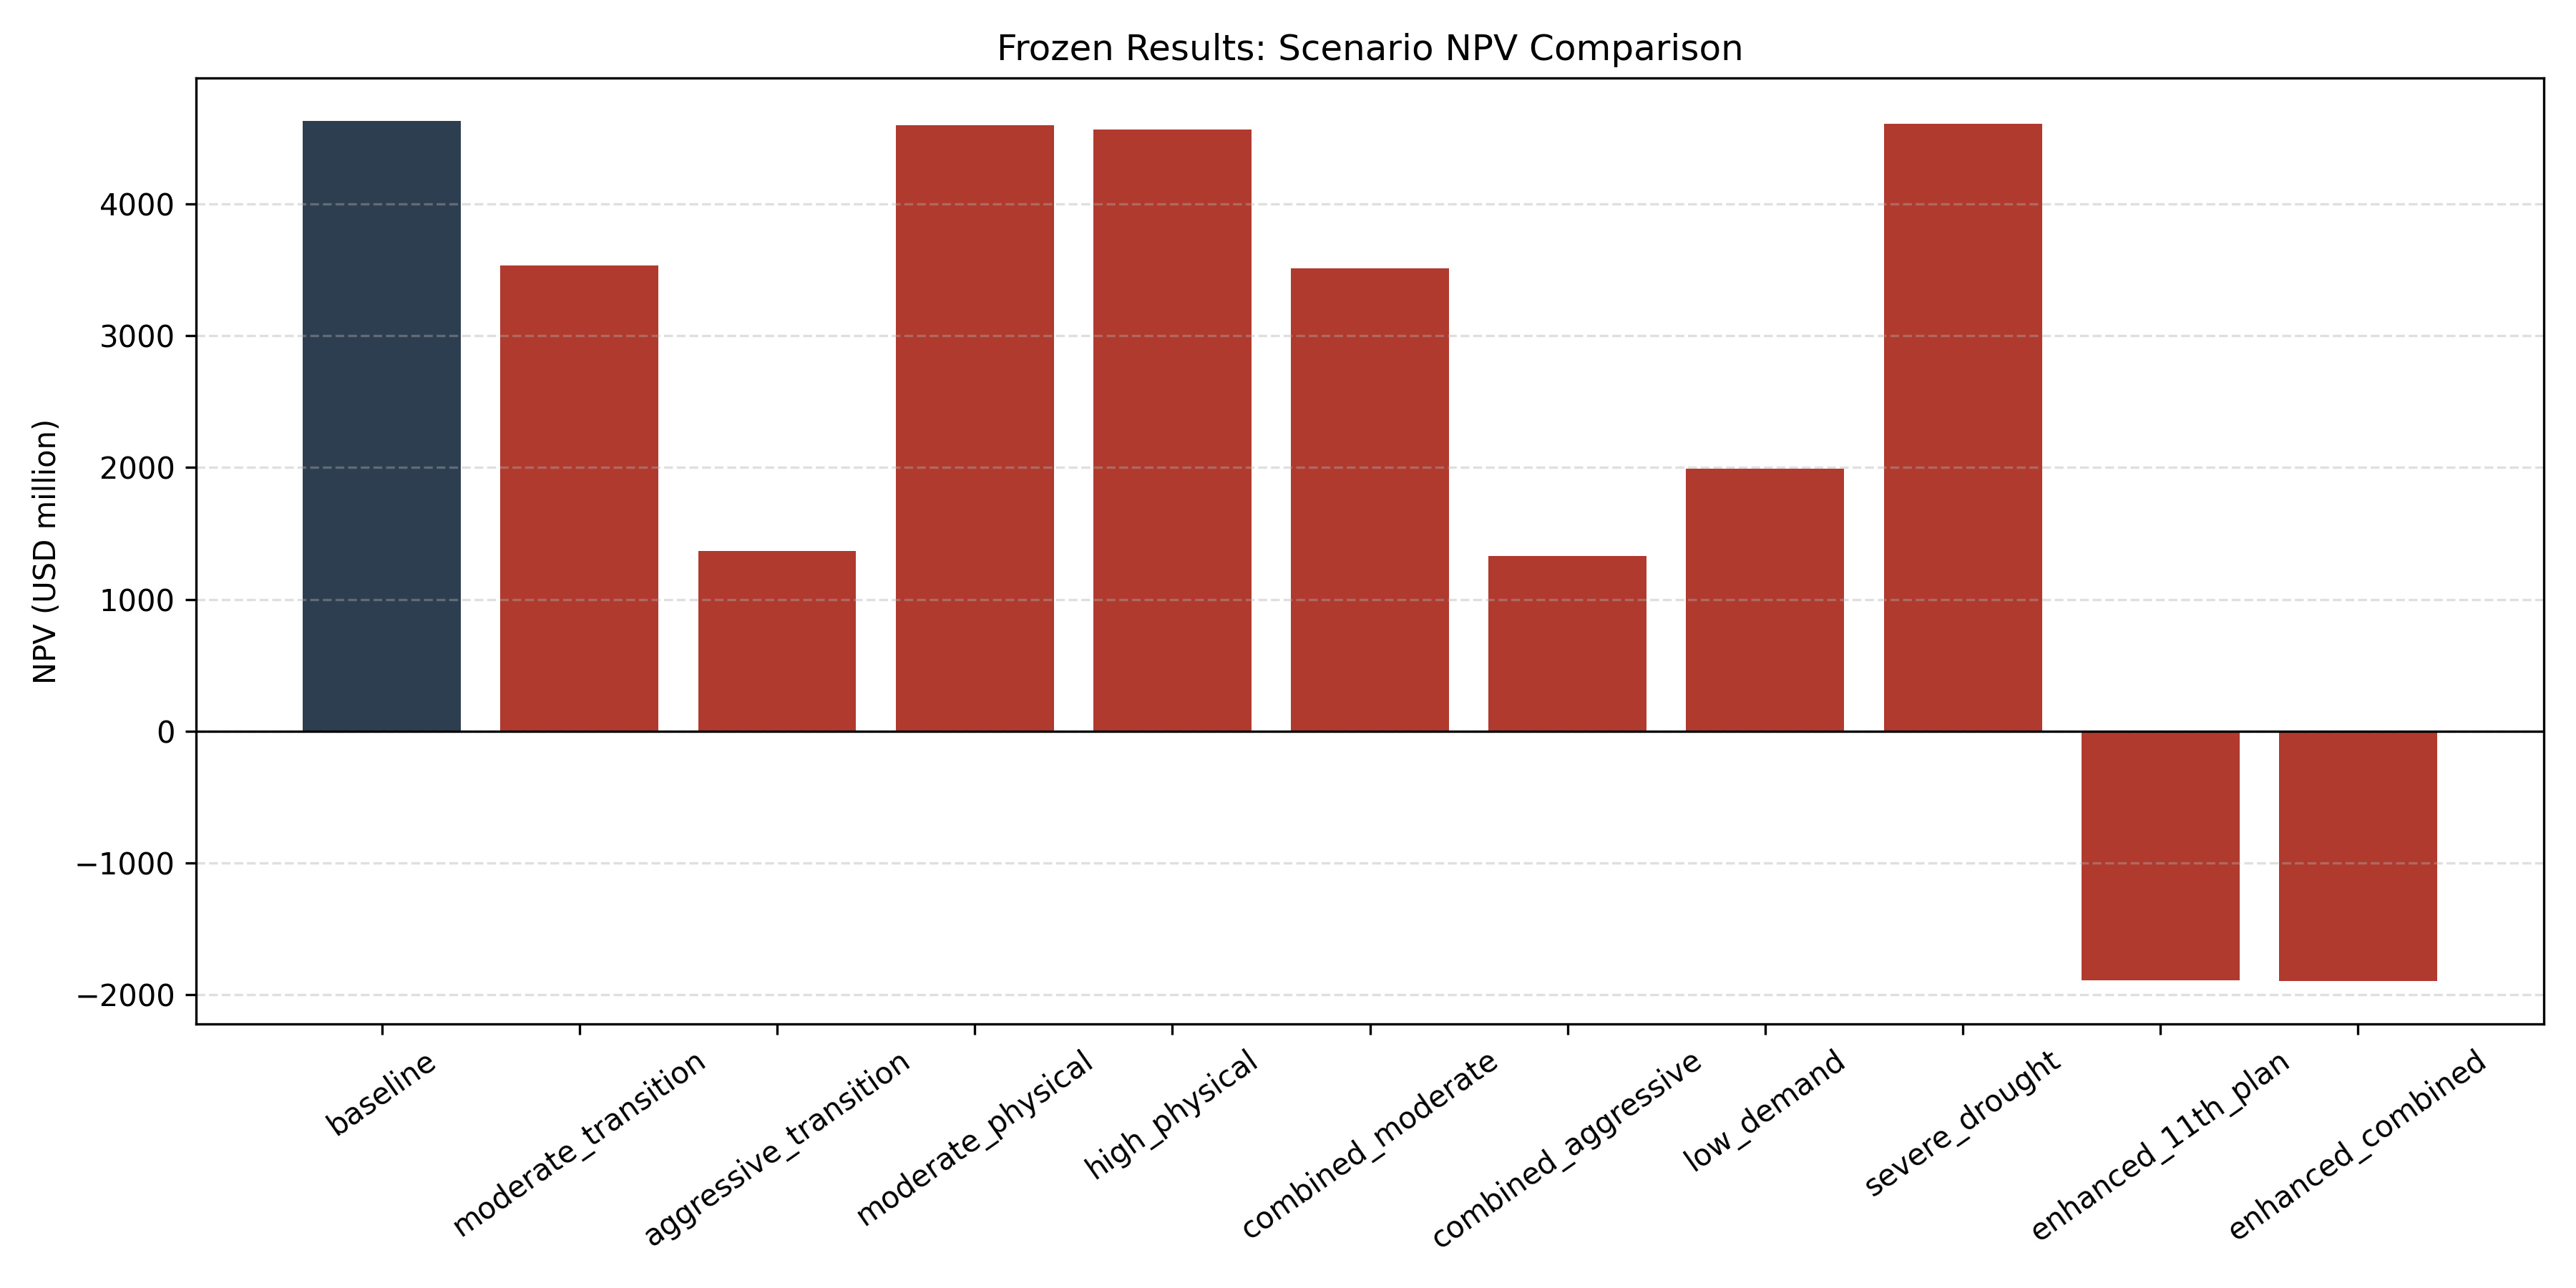
\includegraphics[width=0.95\textwidth]{../03_figures/fig_npv_frozen.png}
    \caption{Frozen scenario NPV comparison.}
\end{figure}

\begin{figure}[h]
    \centering
    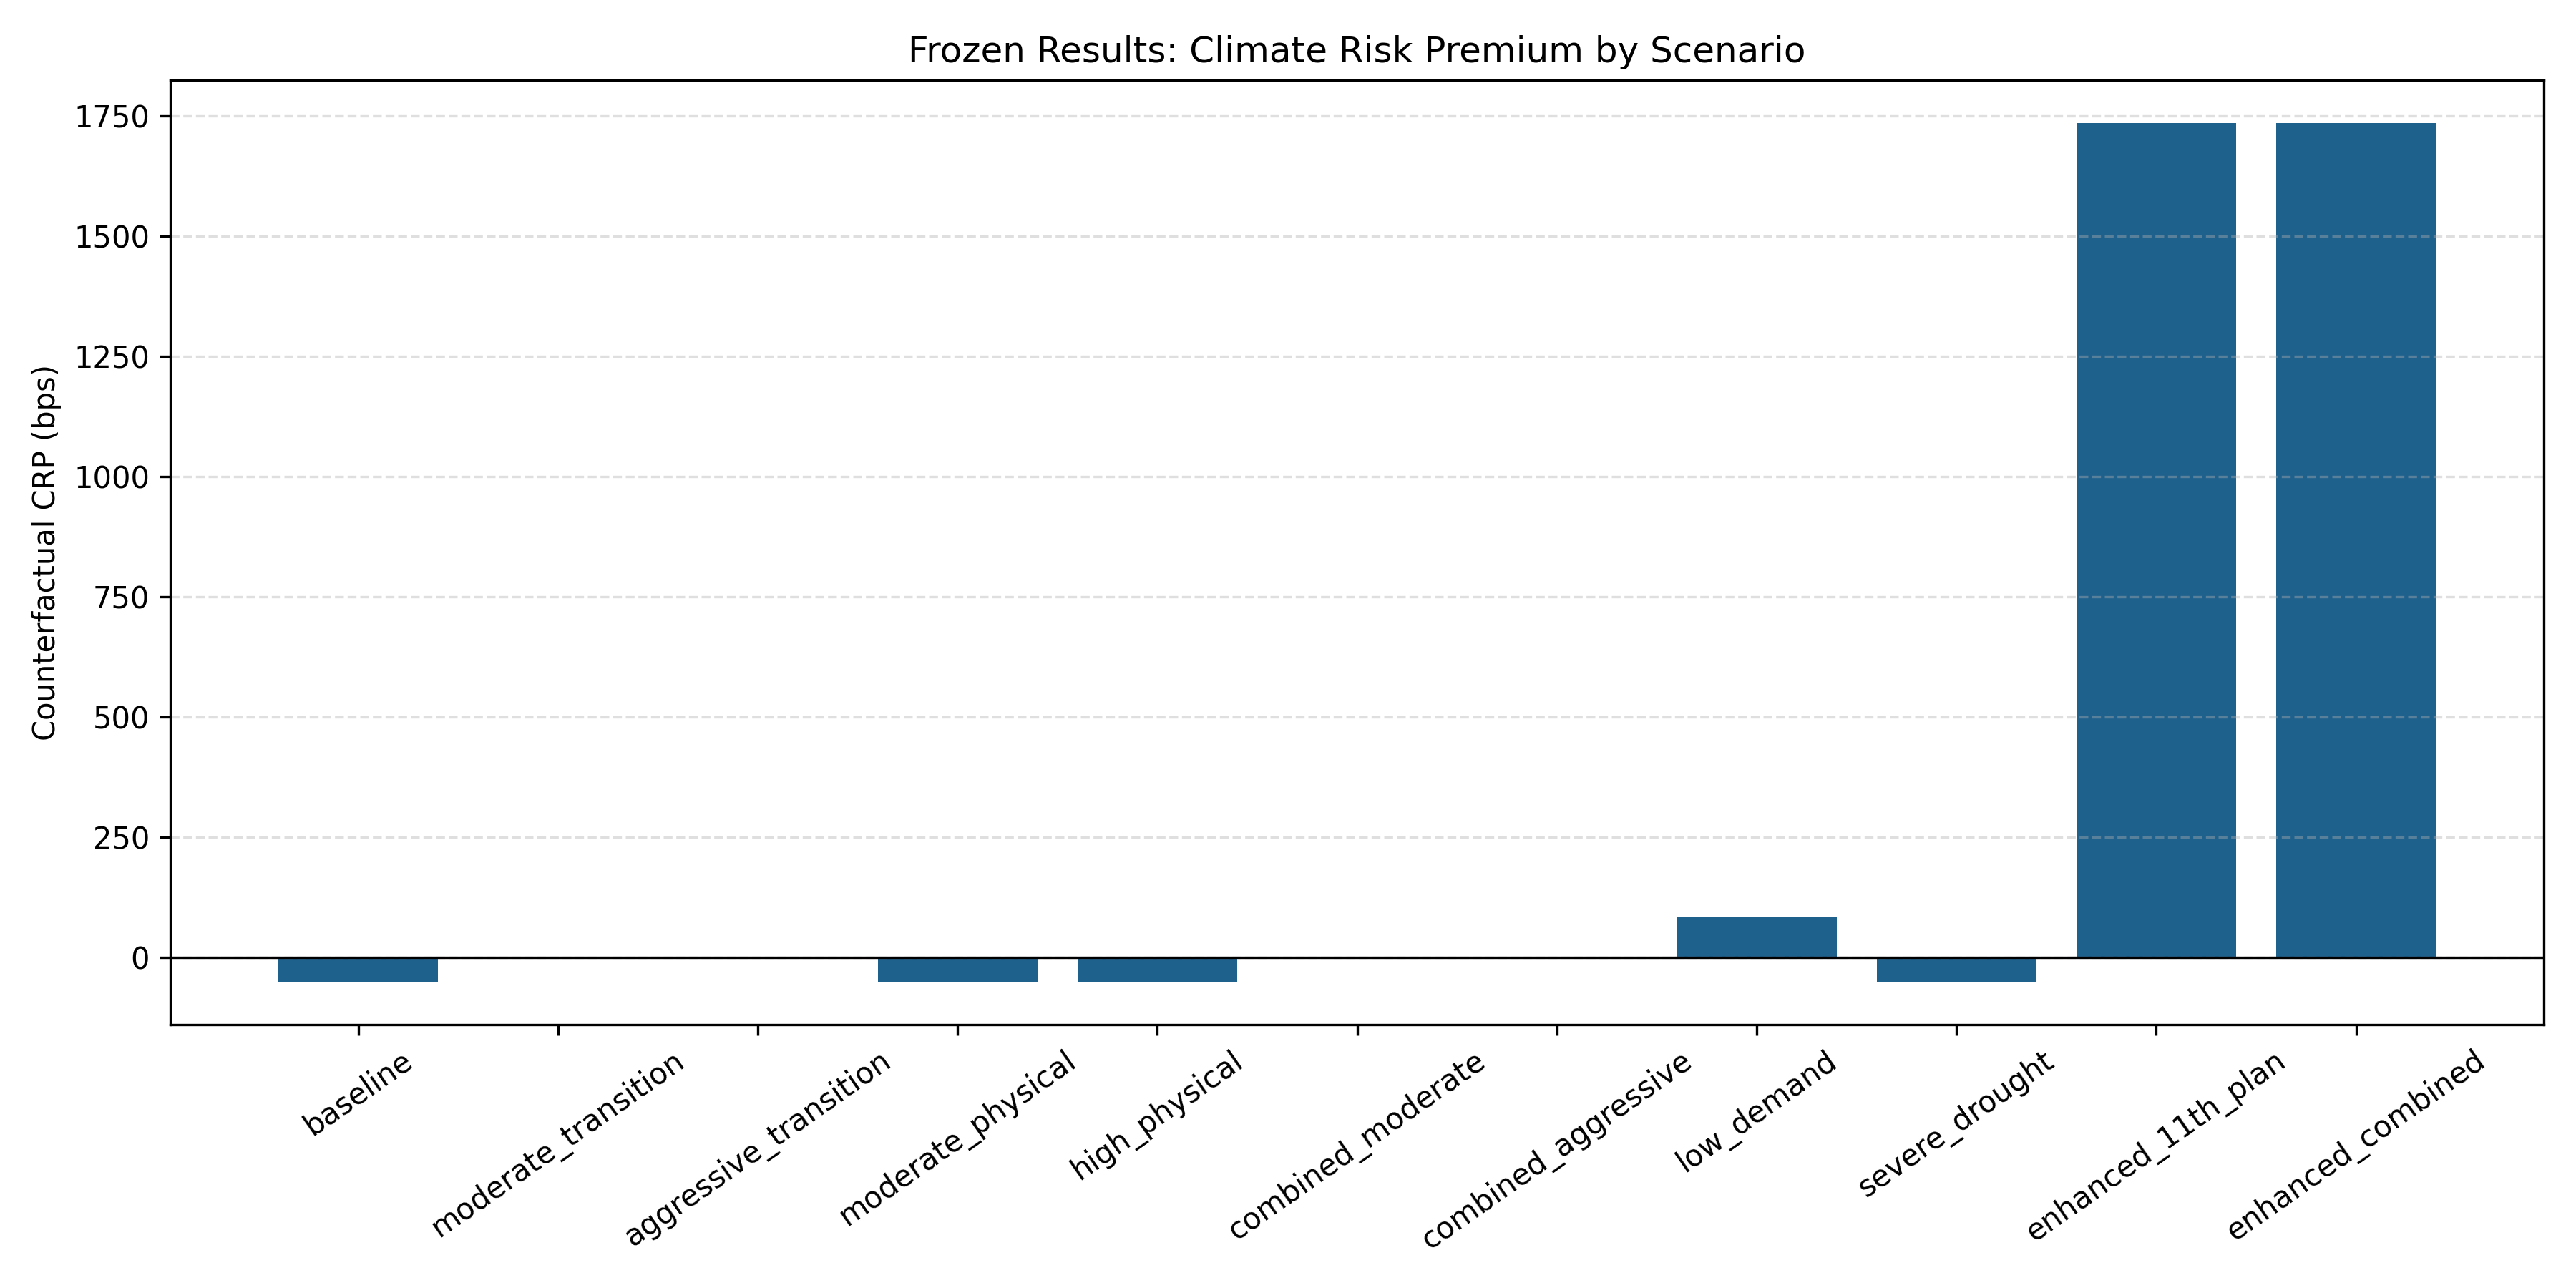
\includegraphics[width=0.95\textwidth]{../03_figures/fig_crp_frozen.png}
    \caption{Frozen counterfactual climate risk premium by scenario.}
\end{figure}

\section{Robustness}
Robustness testing follows a deterministic grid over five axes required by the paper protocol: discount spread ($\pm$200 bps), capacity factor ($\pm$10\%), policy phase-out year shift ($\pm$5 years), carbon-price path (low/base/high), and physical damage multiplier (0.5/1.0/1.5).

Across this grid, the worst NPV stress point is \$\WorstRobustNPV{} million and the best case is \$\BestRobustNPV{} million. The transition-to-physical loss ratio remains \TransitionPhysicalRatio{}, indicating that transition stress remains materially larger than physical-only loss scale in this model configuration.

The placebo removes transition policy shock and applies intensified physical stress. In that placebo, physical-only NPV is \$\PlaceboPhysicalNPV{} million, and transition dominance remains \PlaceboDominance{}. Deterministic-grid dominance is retained in \DominanceSharePct{}\% of tested points.

\begin{figure}[h]
    \centering
    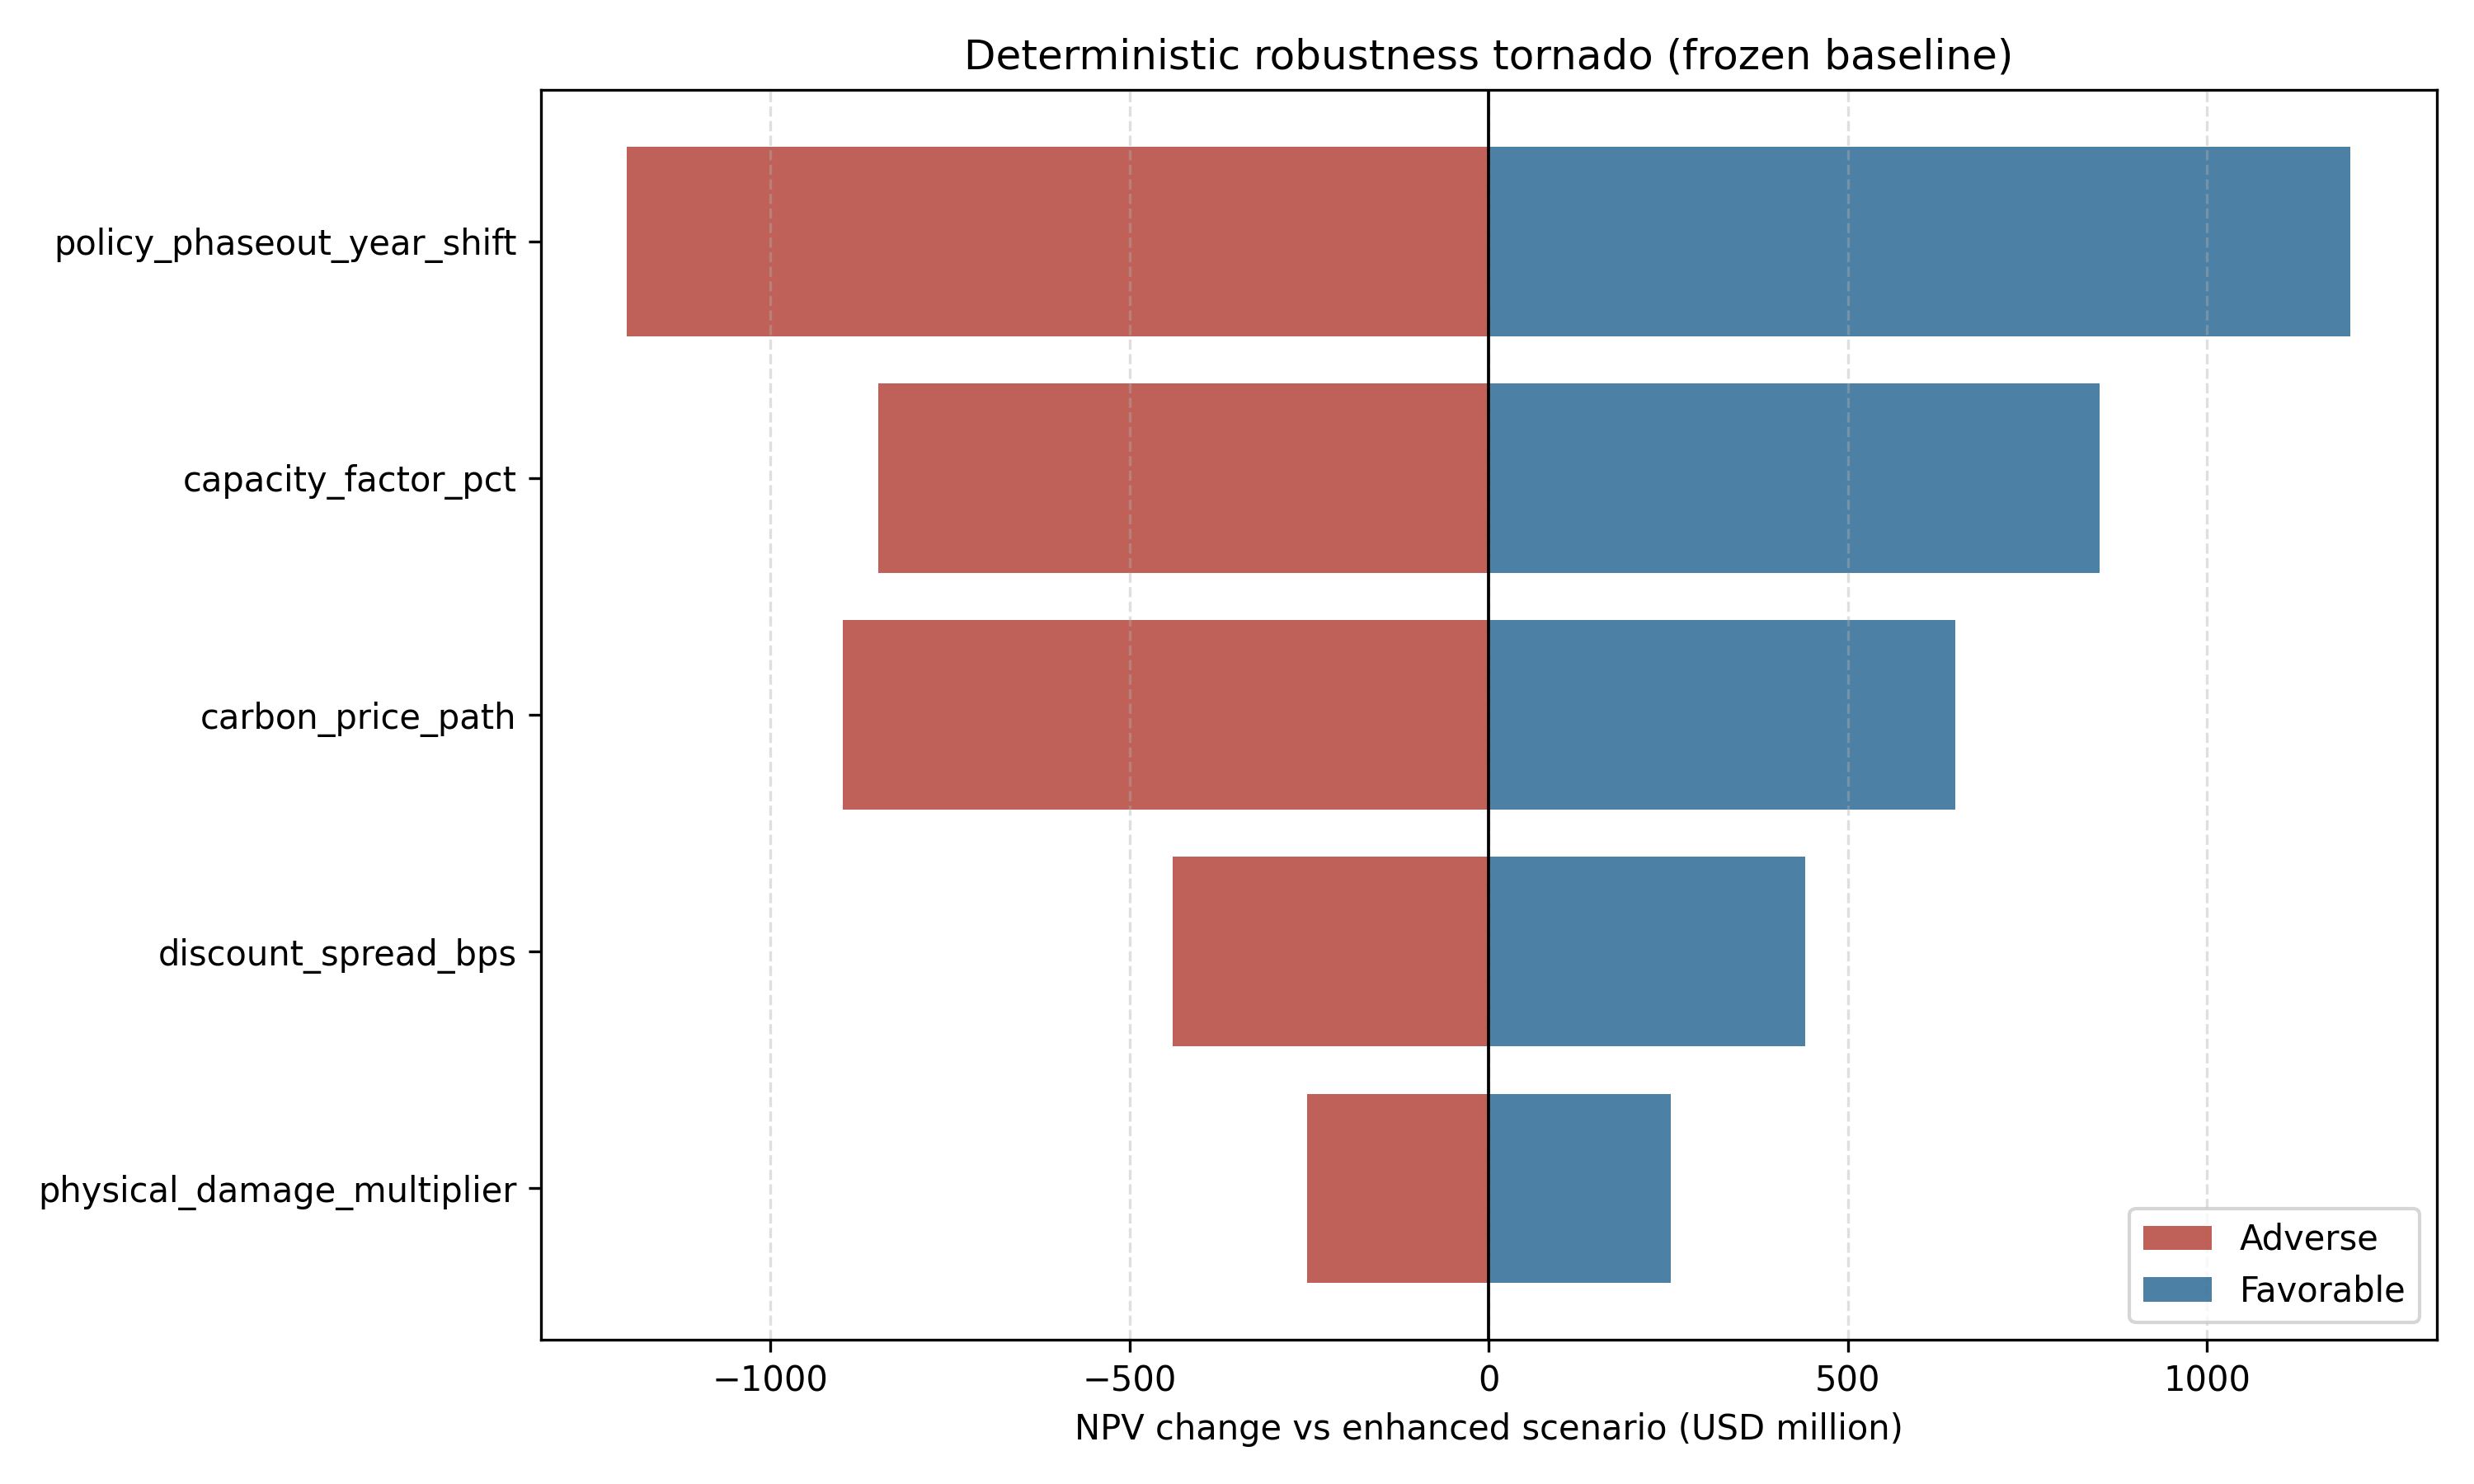
\includegraphics[width=0.95\textwidth]{../03_figures/fig_robustness_tornado.png}
    \caption{Deterministic robustness tornado around enhanced transition baseline.}
\end{figure}

These checks do not prove universal dominance in all model classes. They demonstrate that, within this paper's admissible scenario family and parameter perturbation envelope, the primary conclusion is not driven by a single fragile parameter.

\section{Policy Implications}
Three policy implications follow from the frozen and robustness-consistent evidence.

First, transition-policy clarity is financially consequential at project level. If phase-down trajectories are expected but not reflected in financing assumptions, valuation and credit signals can be systematically biased.

Second, disclosure governance matters as much as model sophistication. Policymakers and public finance institutions increasingly require climate-finance claims that are reproducible and auditable \citep{tcfd2017recommendations}. This study provides a deployable template: scenario contract, frozen outputs, claim-source registry, and manuscript validator.

Third, transition planning and financing design should be discussed jointly. When transition-driven spread penalties become large, policy instruments such as managed retirement contracts, transition-linked refinancing frameworks, and covenant redesign become central to reducing disorderly adjustment risk \citep{ngfs2024,iea2024coal}.

\section{Limitations and Conclusion}
This paper has clear limitations.

It is a single-case study. External validity to other technologies, market structures, and regulatory environments is not automatic \citep{mercure2018stranded}. The appropriate next step is a staged replication strategy across additional assets using the same governance stack.

It is also deterministic in this submission version. We intentionally prioritize transparent sensitivity and placebo tests over probabilistic simulation to reduce assumption opacity. Future work can add uncertainty distributions once parameter priors are documented to publication-grade standards.

Finally, institutional context is deliberately conservative in sourcing. We prioritize source integrity over narrative breadth, which may reduce contextual richness but lowers evidence-risk in peer review.

Within these limits, the conclusion is straightforward. A reproducibility-governed single-case model indicates substantial transition-driven value erosion and financing stress relative to physical-only effects for the Samcheok asset under the frozen admissible scenario set. More broadly, the paper demonstrates a practical standard for climate-finance evidence production in energy policy research: analytical claims should be computationally reproducible, source-traceable, and validator-enforced before submission.

\section*{Declarations}
\textbf{CRediT authorship contribution statement}: Jinsu Park: Conceptualization, Methodology, Software, Validation, Formal analysis, Investigation, Data curation, Writing - original draft, Writing - review \& editing, Visualization.

\textbf{Funding}: No dedicated external grant was used for this submission. Institutional support was provided by PLANiT Institute.

\textbf{Declaration of competing interest}: The author declares no known competing financial interests or personal relationships that could have appeared to influence the work reported in this paper.

\bibliographystyle{elsarticle-harv}
\bibliography{references}

\end{document}
